%%%%%%%%%%%%%%%%%%%%%%%%%%%%%%%%%%%%%%%%%%%%%%%%%%%%%%%%%%%%%%%%%%%%%%%%%%%%%%%%%%%%%%%%%%%%%%%%%%%%%%%%%%%%%%%%%%%%%%%%%%%%%%%%%%%%%%%%%%%%%%%%%%%%%%%%%%%%%%%%%%%
% Written By Michael Brodskiy
% Class: Quantum Mechanics
% Professor: G. Fiete
%%%%%%%%%%%%%%%%%%%%%%%%%%%%%%%%%%%%%%%%%%%%%%%%%%%%%%%%%%%%%%%%%%%%%%%%%%%%%%%%%%%%%%%%%%%%%%%%%%%%%%%%%%%%%%%%%%%%%%%%%%%%%%%%%%%%%%%%%%%%%%%%%%%%%%%%%%%%%%%%%%%

\include{Includes.tex}

\title{Lecture 1}
\date{\today}
\author{Michael Brodskiy\\ \small Professor: G. Fiete}

\begin{document}

\maketitle

\begin{itemize}

  \item Key Features of Quantum Mechanics

    \begin{enumerate}

      \item Probabilistic outcome of measurements

        \begin{itemize}

          \item Compute probabilities \underline{exactly}, and that is the most complete information possible

        \end{itemize}

      \item Dual wave-particle nature of mature

        \begin{itemize}

          \item Which one we observe depends on the experiment performed

        \end{itemize}

      \item Conjugate variables (from classical mechanics) develop ``uncertainty'' relations

        \begin{itemize}

          \item Wave theory relation:

            $$\Delta x\Delta p\geq \hbar$$
            $$\Delta E \Delta t\geq \hbar$$

          \item Classical mechanics is ``contained'' in Quantum mechanics, which includes classical electricity and magnetism

        \end{itemize}

      \item Every particle and object built from particles, including light, falls into one of two classes:

        \begin{itemize}

          \item Fermions (spin is any odd multiple of $\hbar/2$)

            \begin{itemize}
                
              \item Electrons are an example

            \end{itemize}

          \item Bosons (spin is an integer multiple of $\hbar$, including 0)

            \begin{itemize}

              \item Photons are an example

            \end{itemize}

        \end{itemize}

      \item The properties of Quantum mechanics not falling into features 1-4 are largely familiar from classical physics

    \end{enumerate}

  \item Similar but Different

    \begin{itemize}

      \item Every electron has \underline{exactly} the same spin, charge, and mass

      \item Every photon has \underline{exactly} the same spin, charge, and mass

      \item This indicates no inequality among particles of the same type

    \end{itemize}

  \item Time-Evolution in Quantum Mechanics

    \begin{itemize}

      \item Time-evolution is given by the Hamiltonian, $\mathcal{H}$

      \item Hamilton's Equations give us:

        $$\frac{d\vec{q}}{dt}=\frac{\partial \mathcal{H}}{\partial \vec{p}}$$

      \item We may write the Hamiltonian as:

        $$\mathcal{H}=\frac{\vec{p}^2}{2m}\longrightarrow \frac{\partial \mathcal{H}}{\partial \vec{p}}=\frac{\vec{p}}{m}=\vec{v}$$

      \item Alternatively, we may write the force as:

        $$\vec{F}=\frac{d\vec{p}}{dt}=-\frac{\partial \mathcal{H}}{\partial\vec{q}}$$

    \end{itemize}

  \item Stern-Gerlach Experiments

    \begin{itemize}
        
      \item Took place in 1922 with Otto Stern and Walther Gerlach

      \item The act of observing a quantum particle affects its measurable properties in a way foreign to our experience

      \item The experiment looks like this:

        \begin{figure}[H]
          \centering
          \tikzset{every picture/.style={line width=0.75pt}} %set default line width to 0.75pt        

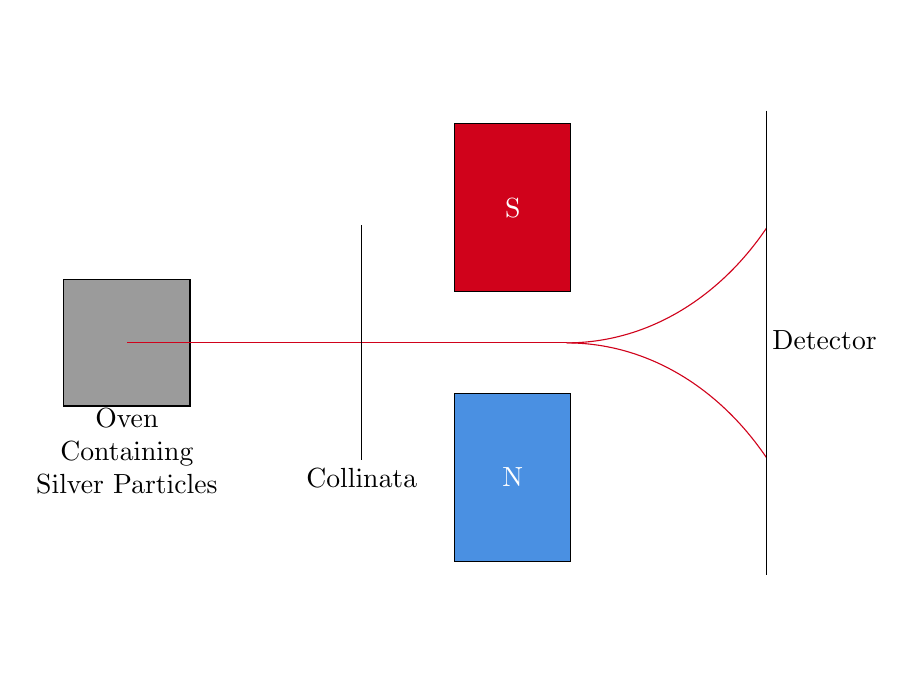
\begin{tikzpicture}[x=0.75pt,y=0.75pt,yscale=-.8,xscale=.8]
%uncomment if require: \path (0,375); %set diagram left start at 0, and has height of 375

%Shape: Square [id:dp14421103605944618] 
\draw  [fill={rgb, 255:red, 155; green, 155; blue, 155 }  ,fill opacity=1 ] (100,128) -- (176,128) -- (176,204) -- (100,204) -- cycle ;
%Straight Lines [id:da6727148484422872] 
\draw [color={rgb, 255:red, 208; green, 2; blue, 27 }  ,draw opacity=1 ]   (279.42,166) -- (138,166) ;
%Straight Lines [id:da8380240359625067] 
\draw    (279.42,95.29) -- (279.42,236.71) ;
%Shape: Rectangle [id:dp32874348023480093] 
\draw  [fill={rgb, 255:red, 208; green, 2; blue, 27 }  ,fill opacity=1 ] (335.42,34) -- (405.42,34) -- (405.42,135.29) -- (335.42,135.29) -- cycle ;
%Shape: Rectangle [id:dp31052784363324215] 
\draw  [fill={rgb, 255:red, 74; green, 144; blue, 226 }  ,fill opacity=1 ] (335.42,196.29) -- (405.42,196.29) -- (405.42,297.58) -- (335.42,297.58) -- cycle ;
%Straight Lines [id:da09102819630459058] 
\draw [color={rgb, 255:red, 208; green, 2; blue, 27 }  ,draw opacity=1 ]   (402.84,166) -- (279.42,166) ;
%Shape: Arc [id:dp14380617240917248] 
\draw  [draw opacity=0] (402.84,166) .. controls (402.84,166) and (402.84,166) .. (402.84,166) .. controls (451.32,166) and (494.63,192.92) .. (523.21,235.14) -- (402.84,355.5) -- cycle ; \draw  [color={rgb, 255:red, 208; green, 2; blue, 27 }  ,draw opacity=1 ] (402.84,166) .. controls (402.84,166) and (402.84,166) .. (402.84,166) .. controls (451.32,166) and (494.63,192.92) .. (523.21,235.14) ;  
%Shape: Arc [id:dp018293912875773533] 
\draw  [draw opacity=0] (402.84,166) .. controls (402.84,166) and (402.84,166) .. (402.84,166) .. controls (451.32,166) and (494.63,139.08) .. (523.21,96.86) -- (402.84,-23.5) -- cycle ; \draw  [color={rgb, 255:red, 208; green, 2; blue, 27 }  ,draw opacity=1 ] (402.84,166) .. controls (402.84,166) and (402.84,166) .. (402.84,166) .. controls (451.32,166) and (494.63,139.08) .. (523.21,96.86) ;  
%Straight Lines [id:da21129461638831382] 
\draw    (523.21,164.43) -- (523.21,305.85) ;
%Straight Lines [id:da4601124961028422] 
\draw    (523.21,26.15) -- (523.21,167.57) ;

% Text Node
\draw (138,204) node [anchor=north] [inner sep=0.75pt]   [align=left] {\begin{minipage}[lt]{70.19pt}\setlength\topsep{0pt}
\begin{center}
Oven \\Containing \\Silver Particles
\end{center}

\end{minipage}};
% Text Node
\draw (279.42,239.71) node [anchor=north] [inner sep=0.75pt]   [align=left] {\begin{minipage}[lt]{42.43pt}\setlength\topsep{0pt}
\begin{center}
Collinata
\end{center}

\end{minipage}};
% Text Node
\draw (370.42,84.64) node  [color={rgb, 255:red, 255; green, 255; blue, 255 }  ,opacity=1 ] [align=left] {S};
% Text Node
\draw (370.42,246.93) node  [color={rgb, 255:red, 255; green, 255; blue, 255 }  ,opacity=1 ] [align=left] {N};
% Text Node
\draw (525.21,164.43) node [anchor=west] [inner sep=0.75pt]   [align=left] {Detector};


\end{tikzpicture}

          \caption{Set Up of Stern-Gerlach Experiment}
          \label{fig:1}
        \end{figure}

      \item Assuming an atom has a monopole moment, $\vec{\mu}$, the potential energy of the interaction with a magnetic field $\vec{B}$ is $E=\vec{\mu}\vec{B}$

      \item Consider a classical description of the atom's moment:

        $$\mu=IA$$

        \begin{itemize}

          \item Where $I$ is the electrical current and $A$ is the area of the loop

        \end{itemize}

      \item A particle of charge $q$ traveling at speed $v$ in a circle of radius $r$ gives us:

        $$\mu=\frac{qvr}{2}=\frac{qL}{2m}$$

        \begin{itemize}

          \item Where $L=mvr$ is the orbitable angular momentum

        \end{itemize}

      \item Particles carry an intrinsic angular momentum, $\vec{S}$, called spin

        $$\vec{\mu}=\frac{gq\vec{S}}{2m}$$

        \begin{itemize}

          \item Where $g$ is the gyroscopic ratio

        \end{itemize}

      \item Noting that silver atoms were used is important, as different atoms give different results. Considering the shell filling of silver, we know that it extends to a singular atom in the $5s$ shell.

        \begin{itemize}

          \item Since the mass of the nucleus $\geq 2000m_e$, we find a ratio of magnetic moments as:

            $$\frac{\vec{\mu}_{nuc}}{\vec{\mu}_{e^-}}<<1$$

          \item Hence, we have $\vec{\mu}_{\text{Ag}}=-g\dfrac{e}{2m_e}\vec{S}$, where $e$ is the magnitude of an electron's charge

          \item This produces a force of $F_z=-g\dfrac{e}{2m_e}S_z\cdot\dfrac{2B_z}{2z}$

          \item Thus, the deflection of the beam in the Stern-Gerlach experiment is a measure of the projection of the intrinsic spin onto the $z$-axis

          \item Note, the heat of the oven randomizes the direction of $\vec{\mu}$, and, classicly, we have $S_z=|\vec{S}|\cos(\theta)$ and should be continuous over an $S_z$ range given by: $-|\vec{S}|\leq S_z\leq |\vec{S}|$

            \begin{itemize}

              \item But, only two beams are observed!

                \begin{itemize}

                  \item Only two $S_z$ components are possible, since $S_z=\pm \hbar/2$

                \end{itemize}

            \end{itemize}

        \end{itemize}

      \item We know:

        $$\hbar\approx=1.0546\cdot10^{-34}[\si{\joule\second}]=6.5821\cdot10^{-16}[\si{eV\second}]$$

        $$\hbar=\frac{h}{2\pi}\text{ (Planck's Constant)}$$

    \end{itemize}

\end{itemize}

\end{document}

